\chapter{Literature Review} 
Various approaches to enable autonomous flight have been proposed in the literature. Some works tackle only perception and build high-quality maps from imperfect measurements, whereas others focus on planning without considering perception errors. Numerous systems that combine online mapping with traditional planning algorithms have been proposed to achieve autonomous flight in previously unknown environments. A taxonomy of prior works is presented in Figure \ref{fig:taxonomy}.

\begin{figure}[h]
	\begin{center}
		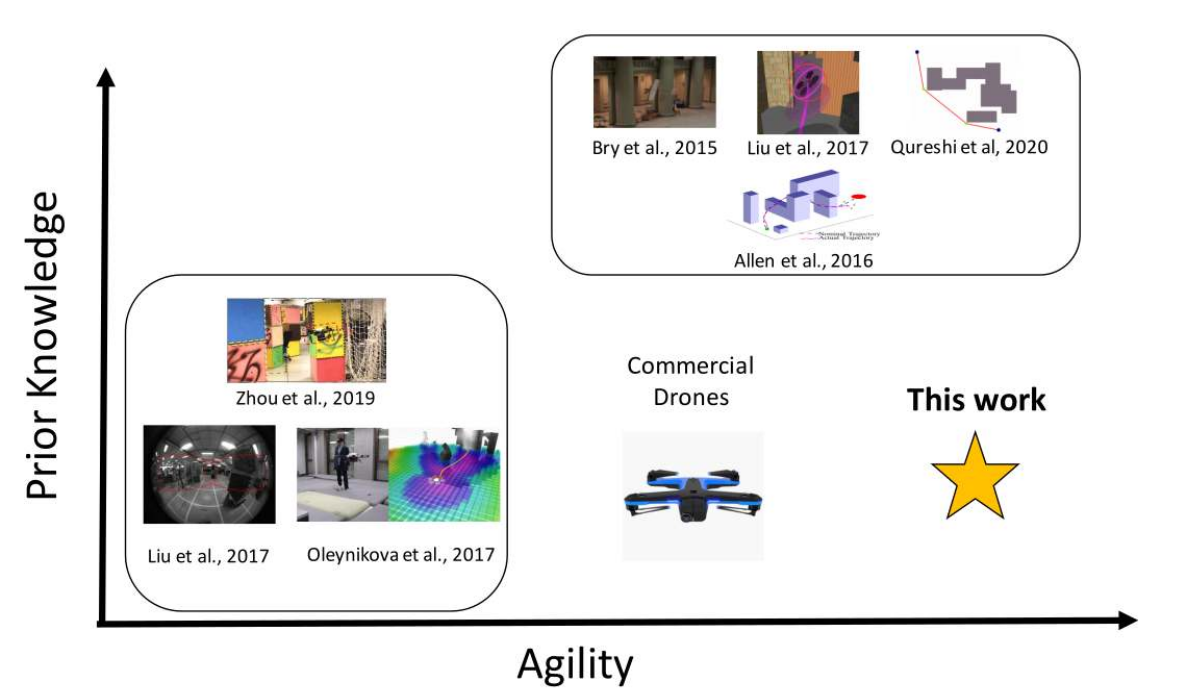
\includegraphics[width=0.75\textwidth]{taxonomy_navigation.png}
		\caption{Taxonomy of prior works}
		\label{fig:taxonomy}
	\end{center}
\end{figure}

\section{Traditional Models}
Traditional methods mainly involve the division of the navigation task into sensing, mapping and planning sub-tasks. The sensors captures the environment details which are then appropriately mapped to calculate the current state of the quadrotor. This information is used to plan the route for the navigation and associated commands are issued to the rotor. Such as system is attractive from an engineering perspective, because it enables parallel progress on each component and makes the overall system interpretable. However, it leads to pipelines that largely neglect interactions between the different stages and thus compound errors. Their sequential nature also introduces additional latency, making high-speed and agile maneuvers impossible. These issues can be mitigated to some degree by careful hand-tuning and engineering via divide-and-conquer principle that has been prevalent in research on autonomous flight. But such a model imposes fundamental limits on the speed and agility that a robotic system can achieve. 

\section{Recent Models}
Some recent works propose to learn end-to-end policies directly from data without explicit mapping and planning stages. These policies are trained by imitating a human, from experience that was collected in simulation, or directly in the real world. Because the number of samples required to train general navigation policies is very high, existing approaches impose constraints on the quadrotor’s motion model with reduced maneuverability and agility. 

More recent work has demonstrated that very agile control policies can be trained in simulation. Such policies can successfully perform acrobatic maneuvers, but can only operate in unobstructed free space and are essentially blind to obstacles in the environment.

\subsection{FastPlanner }
The FastPlanner\cite{fastPlanner} incrementally builds a map from a series of observations and plans a trajectory in this map to reach the goal while avoiding obstacles. It is a novel online motion planning method for quadrotor autonomous navigation. Here, it decouples the online fast motion planning problem as a front-end kinodynamic path searching and a back-end nonlinear trajectory optimization. Kinodynamic path searching is adopted to find a safe, kinodynamic feasible and minimum-time initial path, which is further improved in smoothness and clearance by a gradient based optimization. By utilizing the convex hull property of B-spline, it significantly improves the efficiency and convergent rate of the optimization compared to previous gradient-based planning methods. By representing the trajectory as a non-uniform B-spline, the time allocation according to a given expected flight aggressiveness can be adjusted.

\subsection{Reactive Planner}
Reactive planner\cite{reactive_method} does not build a map but uses instantaneous depth information to select the best trajectory from a set of pre-defined motion primitives based on a cost that encodes collision and progress toward the goal. It makes use of integrated perception and control for robust high-speed quadrotor flight through unknown cluttered environments. Motivated by experiments in which the difficulty of accurate state estimation was a primary limitation on speed, this method forgoes maintaining a map in favor of using only instantaneous depth information in the local frame. This provides robustness in the presence of significant state estimate uncertainty. The probabilistic formulation provides a natural way to integrate reactive obstacle avoidance with arbitrary navigation objectives. It has a motion primitive library which is utilized to compare with a global path-generation and path following approach.


\section{Proposed Model}
An approach to fly a quadrotor at high speeds in a variety of environments with complex obstacle geometry (Figure \ref{fig:navigation real envt}) while having access to only onboard sensing and computation is proposed. By predicting navigation commands directly from sensor measurements, latency between perception and action can be decreased while simultaneously being robust to perception artifacts, such as motion blur, missing data, and sensor noise. 

The policy is exclusively trained in simulation. Stereo matching algorithm\cite{stereoMatching} is utilized to provide depth images as input to the policy, showing a strong similarity of the noise models between simulated and real observations. 

The navigation policy is trained via privileged learning on demonstrations that are provided by a sampling-based expert. The expert uses Metropolis-Hastings\cite{MH_hasting} (M-H) sampling to compute a distribution of collision-free trajectories. This captures the multi-modal nature of the navigation task where many equally valid solutions can exist. The sampler is bias toward obstacle-free regions by conditioning it on trajectories from a classic global planning algorithm\cite{global_planning}.

The neural network policy takes a noisy depth image and inertial measurements as sensory inputs and produces a set of short-term trajectories together with an estimate of individual trajectory costs. The policy adaptively maps the predicted trajectories to the best trajectories that have been found by the sampling-based expert.

\begin{figure}
	\centering
	\begin{subfigure}[b]{\textwidth}
		\centering
		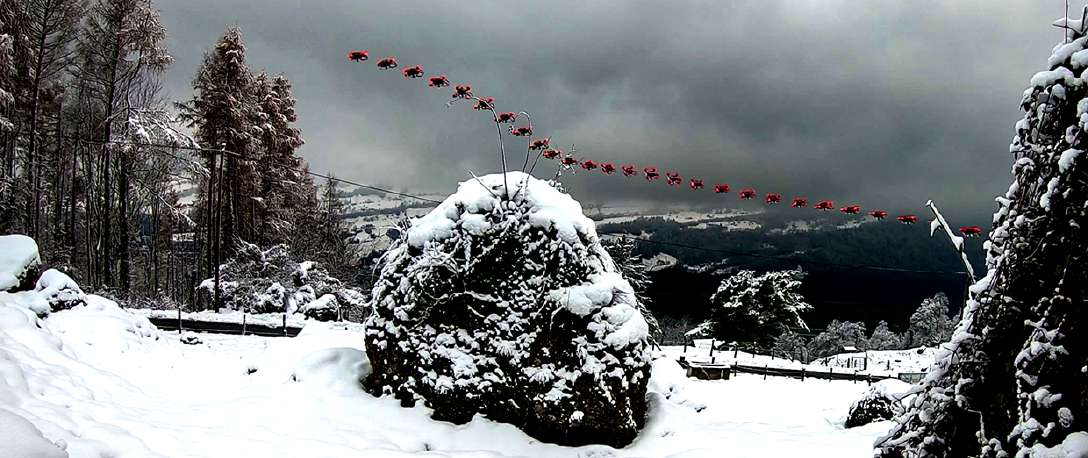
\includegraphics[keepaspectratio=true, width=\textwidth]{Navigation Environment/snow.png}
		\caption{Snowy Environment}
	\end{subfigure}
	\hfill
	\begin{subfigure}[b]{0.48\textwidth}
		\centering
		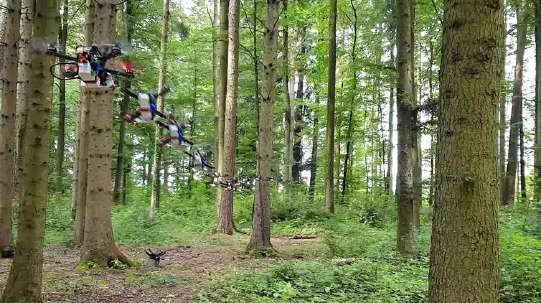
\includegraphics[keepaspectratio=true, width=\textwidth]{Navigation Environment/forest.png}
		\caption{Dense forest}
	\end{subfigure}
	\hfill	
	\begin{subfigure}[b]{0.48\textwidth}
		\centering
		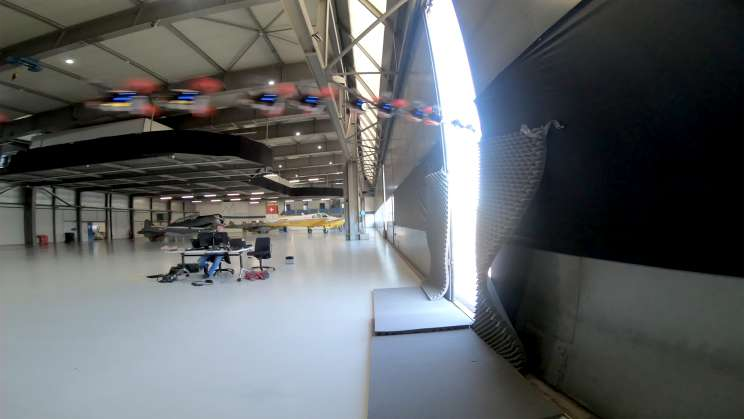
\includegraphics[keepaspectratio=true, width=\textwidth]{Navigation Environment/narrow gap.png}
		\caption{Narrow gaps}
	\end{subfigure}
	\hfill
	\begin{subfigure}[b]{0.48\textwidth}
		\centering
		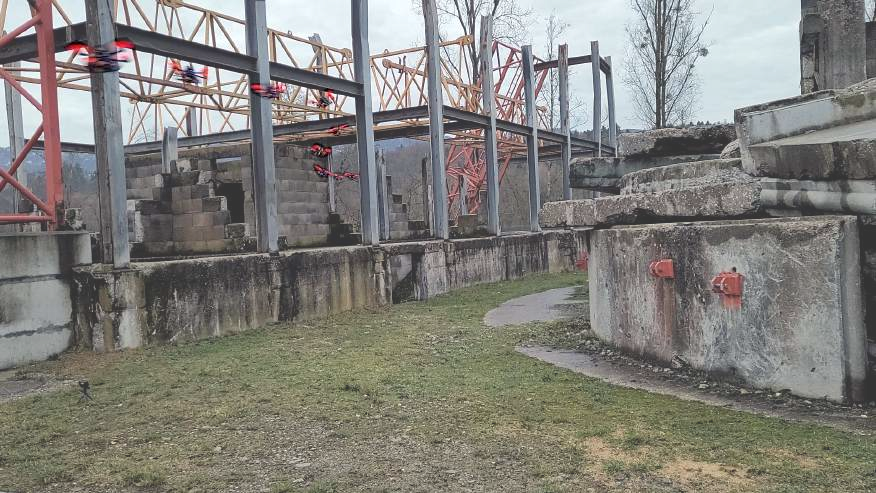
\includegraphics[keepaspectratio=true, width=\textwidth]{Navigation Environment/construction site.png}
		\caption{Construction sites}
	\end{subfigure}
	\hfill
	\begin{subfigure}[b]{0.48\textwidth}
		\centering
		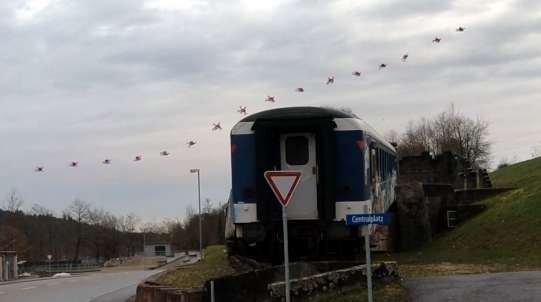
\includegraphics[keepaspectratio=true, width=\textwidth]{Navigation Environment/open space.png}
		\caption{Derailed Train}
	\end{subfigure}
	
	\caption{Time-lapse illustrations of agile navigation}
	\label{fig:navigation real envt}
\end{figure}